\section{Schema concettuale ristrutturato}
%Immagine
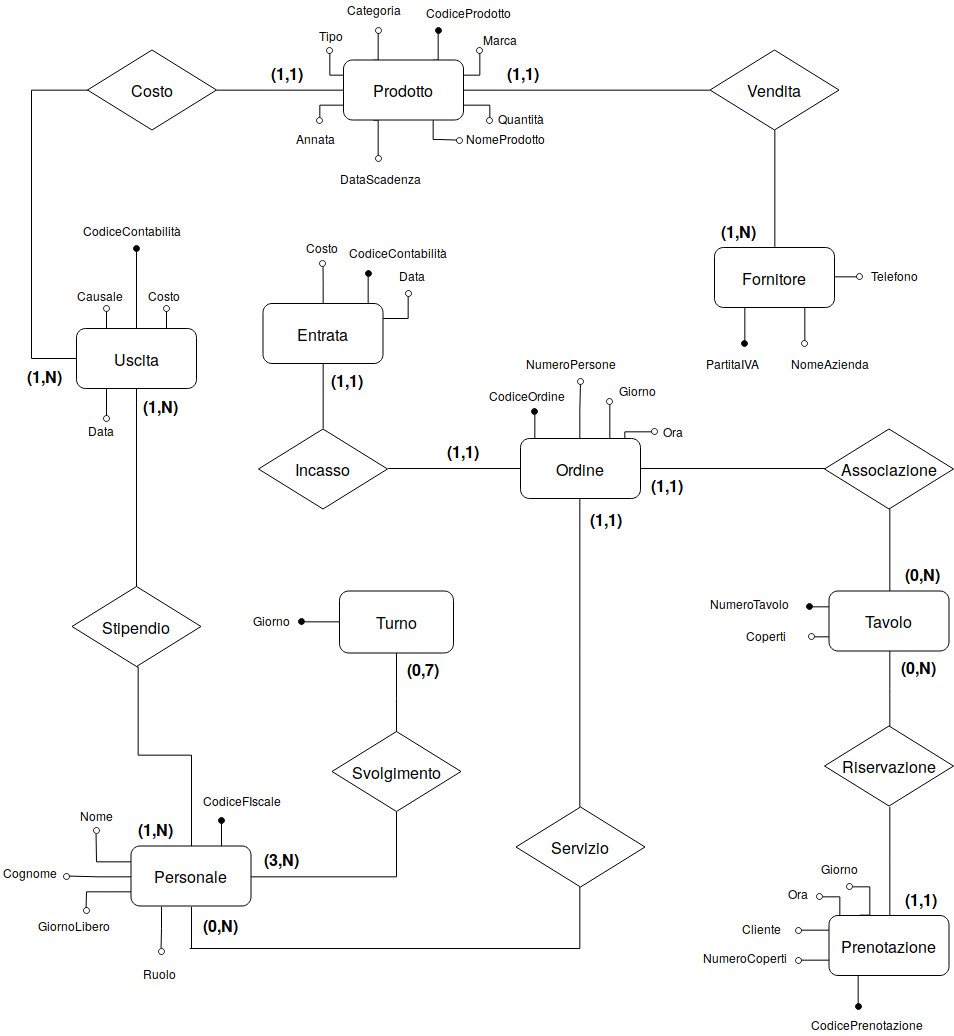
\includegraphics[width=1\textwidth]{doc/Ristrutturato}
\textbf{Eventuali note:}  
\begin{itemize}
    \item Dato che i sistemi tradizionali per la gestione per le basi di dati non consentono di rappresentare direttamente una \textit{generalizzazione} ne tantomeno una gerarchia, risulta necessario trasformare questo costrutto in entità e relazioni. \\
    Per la nostra base di dati si è deciso di utilizzare due dei tre tipi di eliminazione:\\
    Accorpamento delle figlie della generalizzazione nel genitore e accorpamento del genitore della generalizzazione nelle figlie.\\ 
    Il primo metodo è stato utilizzato per l'eliminazione della gerarchia che coinvolge Vino, Superalcolico e Bevanda, per quella che coinvolge Cibo, Bevanda e Prodotto aggiungendo un attributo Categoria che distingue tra cibo e bevanda; il primo metodo viene usato anche per la generalizzazione che comprende Personale, Cuoco, Sommelier e Cameriere, dove in Personale è stato aggiunto un attributo Ruolo.\\
    Il secondo metodo è stato usato per accorpare Contabilità con le figlie Uscita ed Entrata.
    \item I sistemi di gestione di basi di dati richiedono generalmente di specificare una chiave primaria; nei casi in cui esistono entità per le quali sono specificati più identificatori bisogna decidere quali di questi usare come chiave primaria. \\
    Dato che un identificatore composto da uno o pochi attributi è da preferire a identificatori costituiti da molti attributi e per gli stessi motivi, un identificatore interno è da preferire a uno esterno gli \textit{identificatori esterni} delle entità Ordine e Prenotazione vengono sostituiti con CodiceOrdine e CodicePrenotazione.
\end{itemize}

\section{Schema logico}
%Immagine
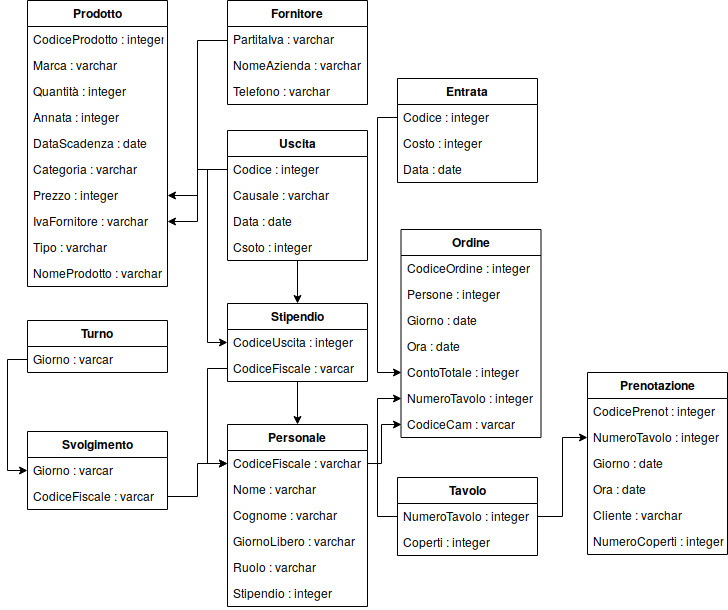
\includegraphics[width=1\textwidth]{doc/schemaLogico}
\subsection{Schema logico-relazionale} %Tabella(Attributi, .. )
\textbf{Fornitore}(\underline{PartitaIVA}, NomeAzienda, Telefono), \\ \smallskip
\textbf{Prodotto}(\underline{CodiceProdotto}, Categoria, Marca, Tipo, Annata, DataScadenza, NomeProdotto, Quantita, IVAFornitore, Prezzo), \\ \smallskip
\textbf{Uscita}(\underline{CodiceUscita},Costo, Data, Causale), \\ \smallskip
\textbf{Stipendio}( \underline{CodiceUscita}, \underline{CodiceFiscale} ), \\ \smallskip
\textbf{Entrata}(\underline{CodiceEntrata}, Costo, Data), \\ \smallskip
\textbf{Personale}(\underline{CodiceFiscale}, Nome, Cognome, Ruolo, GiornoLibero, Stipendio), \\ \smallskip
\textbf{Turno}(\underline{Giorno}), \\ \smallskip
\textbf{Svolgimento}(\underline{Giorno}, \underline{CodiceFiscale}), \\ \smallskip
\textbf{Ordine}(\underline{CodiceOrdine}, NumeroPersone, Giorno, Ora, ContoTotale, NumeroTavolo, CodiceCameriere), \\ \smallskip 
\textbf{Tavolo}(\underline{NumeroTavolo}, Coperti), \\ \smallskip
\textbf{Prenotazione}(\underline{CodicePren}, NumeroCoperti, Cliente, Giorno, Ora, NumeroTavolo)

\section{Lista dei vincoli di integrità referenziale}
\begin{itemize}
    \item Fra l'attributo PartitaIVA della relazione Fornitore e l'attributo IVAFornitore della relazione Prodotto.
    \item Fra l'attributo CodiceUscita della relazione Uscita e l'attributo Prezzo della relazione Prodotto.
    \item Fra l'attributo CodiceUscita della relazione Uscita e la relazione Stipendio.
    \item Fra l'attributo CodiceFiscale della relazione Stipendio e la relazione Personale.
    \item Fra l'attributo CodiceEntrata della relazione Entrata e l'attributo ContoTotale della relazione Ordine.
    \item Fra l'attributo Giorno della relazione Turno e la relazione Svolgimento.
    \item Fra l'attributo CodiceFiscale della relazione Svolgimento e la relazione Personale.
    \item Fra l'attributo CodiceFiscale della relazione Personale e l'attributo CodiceCameriere della relazione Ordine.
    \item Fra l'attributo NumeroTavolo della relazione Tavolo e la relazione Ordine.
    \item Fra l'attributo NumeroTavolo della relazione Tavolo e la relazione Prenotazione.
\end{itemize}
